\begin{comment}
\begin{fichacatalografica}
	\vspace*{\fill}
	\hrule
	\begin{center}
	\begin{minipage}[c]{12.5cm}

	\imprimirautor

	\hspace{0.5cm} \imprimirtitulo / \imprimirautor. -- \imprimirlocal,
	\imprimirdata-

	\hspace{0.5cm} \pageref{LastPage} p. : il. (algumas color.) ; 30 cm.\\
	\hspace{0.5cm} \imprimirorientadorRotulo~\imprimirorientador\\
	\hspace{0.5cm}
	\parbox[t]{\textwidth}{\imprimirtipotrabalho~--~\imprimirinstituicao,
	\imprimirdata.}\\

	\hspace{0.5cm}
		1. Paradigma Orientado a Notificações. 2. Desenvolvimento Orientado a
  Testes. 3. Programação Genérica. 4. C++ Moderno. I. Linhares, Robson Ribeiro;
  Simão, Jean Marcelo. II. Universidade Tecnológica Federal do Paraná IV.
  \imprimirtitulo\\

	\hspace{8.75cm} CDU 00:000:000.0\\

	\end{minipage}
	\end{center}
	\hrule
\end{fichacatalografica}
\cleardoublepage
\end{comment}

% Insira aqui a folha de aprovação! \includepdf{folhadeaprovacao_final.pdf}

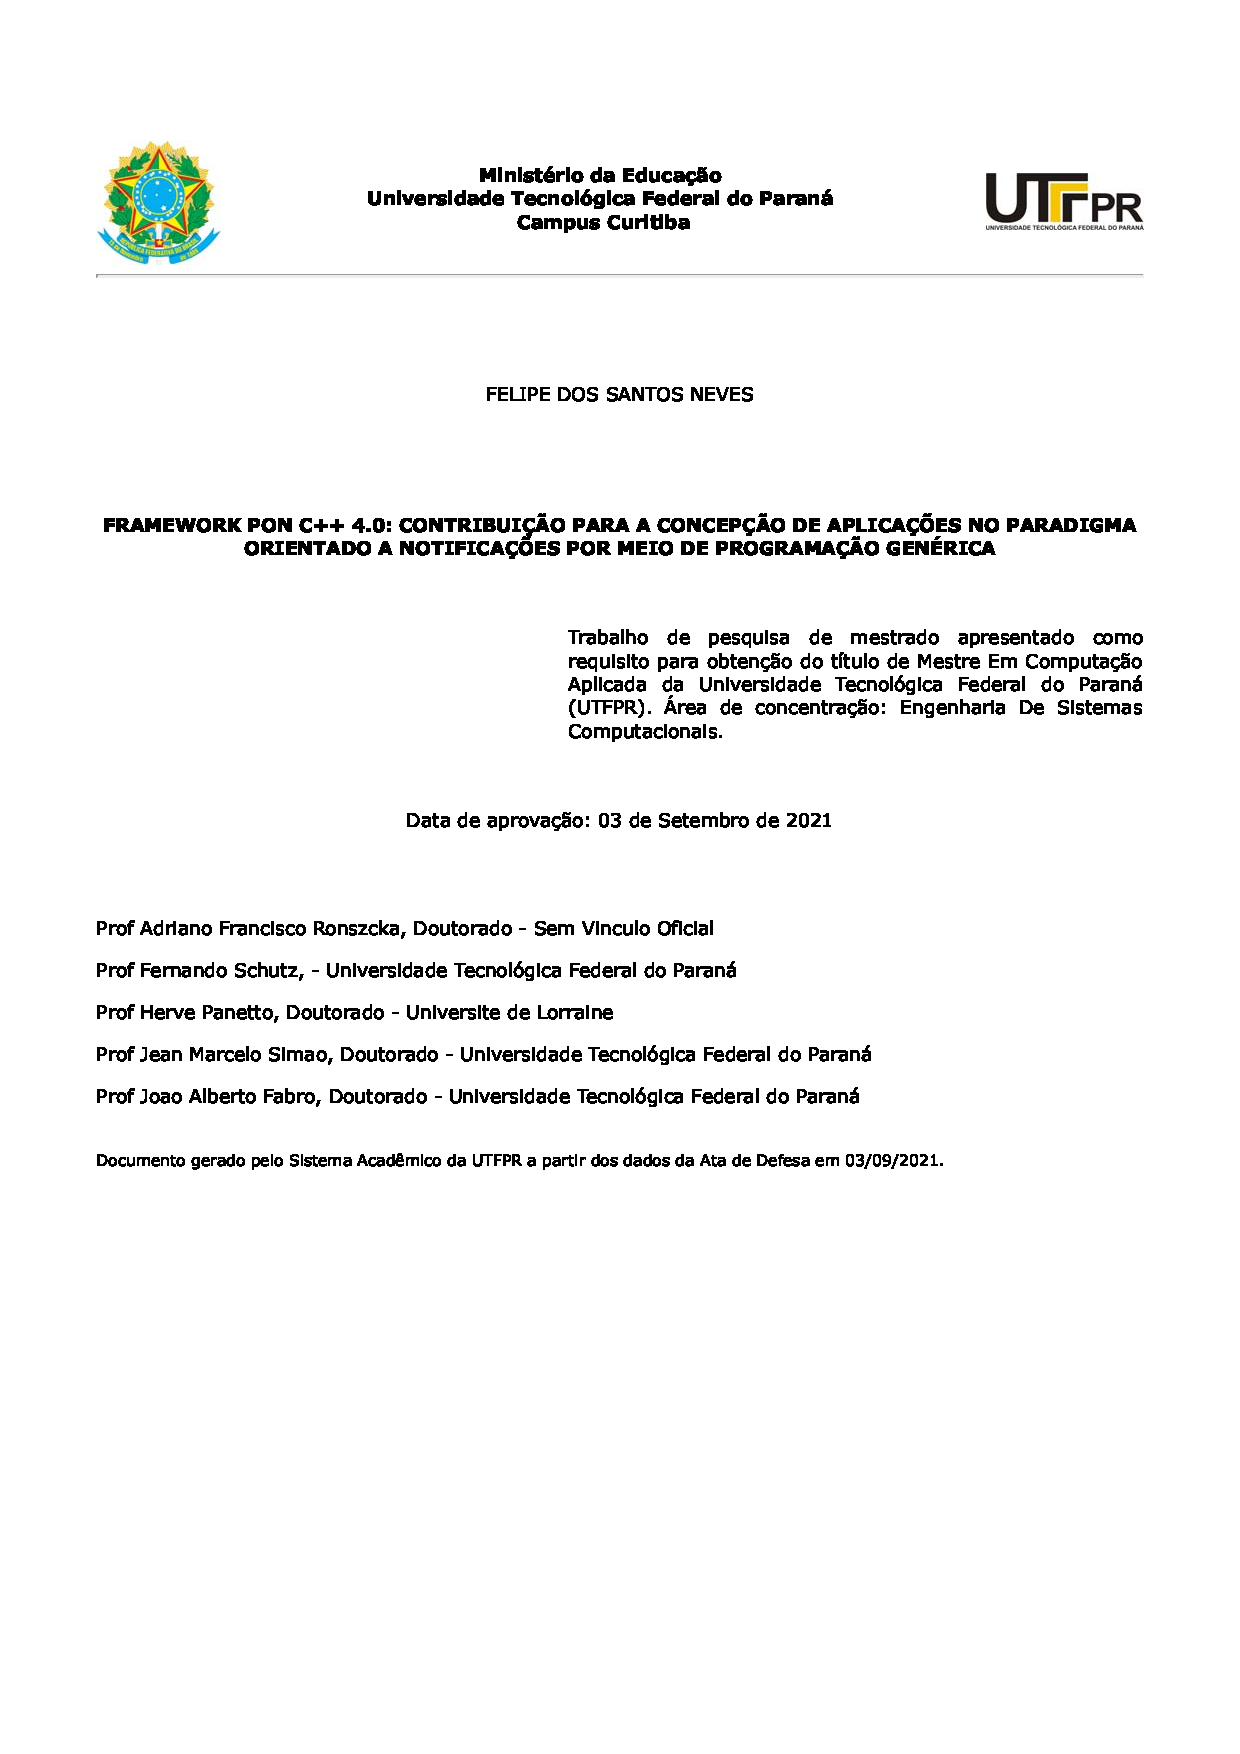
\includepdf[scale=1]{../extra/aprovacao.pdf}

\begin{dedicatoria}
\null
\vfill
\begin{flushright}
Dedico esse trabalho aos meus pais,\\
que me deram a dádiva da educação, \\
sem o qual nada seria possível.
\end{flushright}


\end{dedicatoria}

\begin{agradecimentos}

Sou eternamente grato a toda a minha família, especialmente aos meus pais,
Fernando e Soraya, que acreditaram sempre no meu potencial e me apoiaram em
todas as minhas decisões. Agradeço também a minha esposa Thaís, por todo o amor,
carinho e principalmente paciência durante os períodos em que mais precisei.

Agradeço também a todos os meus professores e colegas de trabalho que tiveram um
impacto na minha carreira, em particular a Felipe Calliari e Luiz Duma que
também acreditaram em meu potencial e me deram a oportunidade de iniciar minha
carreira como desenvolvedor de \textit{software}.

Agradeço aos professores orientadores Dr. Jean Marcelo Simão e Dr. Robson
Ribeiro Linhares por todo o apoio, dedicação e paciência durante o
desenvolvimento deste trabalho. Por fim, agradeço também aos membros da banca Dr. João
Alberto Fabro, Dr. Fernando Schütz, Dr. Adriano Francisco Ronszcka e Dr. Hervé Panetto, por
disponibilizar seu valioso tempo na avaliação deste trabalho.

É imensurável a minha gratidão a todas as pessoas que me ajudaram nessa jornada.
Deixo registrado também meu agradecimento a todos aqueles que, de alguma forma
ou outra, contribuíram para a realização deste trabalho.

\end{agradecimentos}

\begin{epigrafe}
\vspace*{\fill}
\begin{flushright}
\textit{
``Each of us is carving a stone,\\
erecting a column, or cutting \\
a piece of stained glass \\
in the construction of something \\
much bigger than ourselves.'' \\
(Adrienne Clarkson) \\
}
\textit{
``Cada um de nós está a esculpir \\
uma pedra, a erguer uma coluna, \\
ou a cortar um pedaço de vidro \\
manchado na construção de algo \\
muito maior do que nós próprios.'' \\
(Adrienne Clarkson) \\
}
\end{flushright}
\end{epigrafe}

\begin{resumo}

O Paradigma Orientado a Notificações (PON) é uma nova abordagem para a
construção de sistemas computacionais. O PON propõe a computação por meio de um
modelo de entidades reativas desacopladas que interagem por meio de notificações
pontuais, dentre as quais se divide e separa a computação facto-execucional da
computação lógico-causal. Com isso é possível reduzir ou eliminar redundâncias
temporais e estruturais, comuns em outros paradigmas de programação, que podem
afetar o desempenho dos programas. Ainda, o desacoplamento intrínseco entre as
entidades do PON facilita a construção de sistemas concorrentes e/ou
distribuídos. Além disso, a estrutura orientada a regras do PON tende a
facilitar o desenvolvimento por permitir programar em alto nível de abstração. O
PON apresenta várias materializações em \textit{software}, sendo as mais maduras
tecnologicamente aquelas que se dão por meio de \textit{frameworks},
desenvolvidos em diferentes linguagens de programação. Dentre estes
\textit{frameworks} o que apresenta o maior grau de maturidade e estabilidade é
o \textit{Framework} PON C++ 2.0. Entretanto, o \textit{Framework} PON C++ 2.0
ainda apresenta certas limitações, como excessiva verbosidade, baixa
flexibilidade de tipos e baixa flexibilidade algorítmica. Nesse contexto este
trabalho propõe o desenvolvimento de um novo \textit{framework}, denominado
\textit{Framework} PON C++ 4.0, com o objetivo de remover as limitações
presentes no \textit{Framework} PON C++ 2.0, bem como as imperfeições do
\textit{Framework} PON C++ 3.0  que envolve \textit{multithread/multicore}, de
forma a melhorar a usabilidade do PON e seu desempenho neste âmbito. O
\textit{Framework} PON C++ 4.0 é desenvolvido utilizando técnicas de programação
genérica, por meio de recursos adicionados nas versões do padrão ISO C++11,
C++14, C++17 e C++20, bem como aplicando o método de desenvolvimento orientado a
testes. Esta dissertação de mestrado apresenta os resultados obtidos com a
implementação do \textit{Framework} PON C++ 4.0 por meio de um conjunto de
aplicações pertinentes, tanto em ambiente \textit{single thread} quanto
\textit{multithread}/\textit{multicore}. Tais aplicações são um sistema de
sensores e uma aplicação de controle automatizado de tráfego, oriundos do grupo
de pesquisa, e dos algoritmos \textit{Bitonic Sort} e \textit{Random Forest}
oriundos da literatura. Tais aplicações foram executadas e comparadas em termos
de desempenho com as mesmas aplicações implementadas no \textit{Framework} PON
C++ 2.0, \textit{Framework} PON Elixir/Erlang e também implementações no
Paradigma Orientado a Objetos (POO) em linguagem de programação C++ e Paradigma
Procedimental (PP) em linguagem de programação C. Como resultado destas
comparações, o novo \textit{Framework} PON C++ 4.0 se mostra superior ao
\textit{Framework} PON C++ 2.0 tanto em tempo de execução como consumo de
memória nos cenários avaliados, além de apresentar balanceamento de carga
comparável aos do \textit{Framework} PON Elixir/Erlang em ambiente
\textit{multicore}. As melhorias na usabilidade são adicionalmente avaliadas e
atestadas pelo \textit{feedback} de desenvolvedores do PON. 

\vspace{\onelineskip}
Palavras-chaves: Paradigma Orientado a Notificações, \textit{Framework} PON C++ 4.0, Programação Genérica, C++
Moderno, Desenvolvimento Orientado a Testes.

\end{resumo}

\begin{resumo}[Abstract]

The Notification-Oriented Paradigm (NOP) is a new approach to the construction
of computer systems. The NOP proposes computability by means of reactive and
decoupled entities model that interact by means of punctual notifications,
separating fact-executional from logic-causal computing. With this it is
possible to reduce or eliminate temporal and structural redundancies, common in
other programming paradigms, which can affect program performance. Still, the
intrinsic decoupling between NOP entities facilitates the construction of
concurrent and/or distributed systems. Moreover, the rule-oriented structure of
the NOP tends to ease development by allowing programming at a high level of
abstraction. NOP presents several materializations in software, being the
most mature technologically those that occur through frameworks, developed in
different programming languages. Among these frameworks, the one that presents
the highest degree of maturity and stability is the C++ Framework NOP 2.0.
However, the C++ Framework NOP 2.0 still has certain limitations, such as
excessive verbosity, low type flexibility and low algorithmic flexibility. In
this context, this work proposes the development of a new framework, named C++
Framework NOP 4.0, with the objective of removing the limitations present in the
C++ Framework NOP 2.0, as well as the imperfections of the C++ Framework NOP 3.0
that involves multithread/multicore, in order to improve the usability of the
NOP and its performance in this regard. The C++ Framework NOP 4.0 is developed
using generic techniques, by means of features added in the ISO C++11 C++14,
C++17 and C++20 and applying the test-driven development methodology. This
master's thesis presents the results obtained with the implementation of the C++
Framework NOP 4.0 through a set of relevant applications, such as the sensor
application, traffic light control application, and the algorithms Bitonic Sort
and Random Forest, both in a single thread and multithread/multicore
environment. These applications were executed and compared in terms of
performance against the same applications implemented with the C++ Framework NOP
2.0, Elixir/Erlang Framework NOP and also implementations in the Object-Oriented
Paradigm (OOP) in the C++ programming language and Procedural Paradigm (PP) in
the C programming language. As a result of these comparisons, the new C++
Framework NOP 4.0 proves to be superior to C++ Framework NOP 2.0 in both runtime
and memory consumption in the evaluated scenarios, besides presenting CPU
utilization levels comparable to the Framework Elixir/Erlang Framework
NOP multicore environment. Usability improvements are additionally
evaluated and attested by feedback from NOP developers.

\vspace{\onelineskip}
Key-words: Notification-Oriented Paradigm, C++ Framework NOP 4.0, Generic Programming, Modern C++, Test
Driven Development.
\end{resumo}
